% NOTA: las lineas que comienzan con % son comentarios, se ignoran por el compilador de latex

% NOTA 2: todo lo que venga al lado con un \usepackage{} son paquetes que deben estar instalados para que el texto compile. Si no están instalados, van a obtener errores del tipo 'package.sty not found' o 'can't found blabla.sty'. Para instalarlos, pueden usar el package manager de su distro de latex (en MikTex se llama Package Manager si mal no recuerdo, y en TexLive deberían poder acceder aél mediante 'tlmgr --gui' en consola, no sé si en win tiene acceso directo)  

% NOTA 3: cuando se sientan confiados, borren los comentarios excesivos y copien el preámbulo a todos sus informes sin pensarlo dos veces

% NOTA 4: siempre compilar dos veces. Latex necesita que compiles dos veces para poner bien todos los links a ecuaciones, figuras, referencias, etc.

\documentclass[12pt,a4paper]{article} 
% documentclass determina algunos parametros generales del documento. En primer lugar se determina el tamanio de letra, en este caso, 12pt (10pt por default). Ademas se determina el tipo de hoja en el cual queremos acomodar lo que escribimos, en este caso, a4. Podemos agregar otras opciones como por ejemplo twocolumn si deseamos un documento en 2 columnas. Finalmente determinamos el tipo de documento que queremos generar (article para articulos, report para reportes, book para libros etc etc) 

% los paquetes que vienen a continuación, siempre se cargan en ese orden, primero fontenc y después inputenc (para más información 'latex inputenc fontenc' en google)
\usepackage[T1]{fontenc}      
% esto es la codificación de salida (por decirlo de una manera amena n odel todo correcta, el abecedario que va a tener el pdf)

\usepackage[utf8]{inputenc}   
% esto es la codificación que usas vos para escribir en el editor (el abecedario que tiene tu teclado+sistema operativo, otra vez es una manera amena no del todo correcta)

\usepackage[spanish]{babel}   
% para trabajar en castellano necesitamos este paquete

\usepackage{graphicx}  
% Esto es necesario para ver el grafico de la mandarina.

\usepackage{multirow} 
%paquete para poder hacer filas múltiples en tablas

\usepackage{amsmath,amsthm,amssymb}
% símbolos matemáticos especiales, conviene dejarlo siempre

\usepackage{hyperref}
% permite insertar links dentro del texto, que linkeen al mismo texto (indice, figuras, ecuaciones) o a páginas web

\usepackage{subfigure}
% para poner subfiguras (una figura, con figuras a y b; o a, b, y c; o tantas como gusten)

\usepackage{float}
% ESENCIAL para poder controlar el posicionamiento de figuras y tablas (latex pone las figuras donde quiere en base a criterios como minimizar la cantidad de hojas, y no siempre es bueno eso)

\usepackage{geometry}
% permite cambiar el layout de la hoja

\geometry{left=2.0cm, top=1.5cm, right=2.0cm, bottom=2.0cm}
% márgenes cambiado con el paquete geometry

\renewcommand{\thesection}{\Roman{section}}
% con esto cambian el enumarado de secciones a números romanos, pueden comentarlo si no les gusta

%Título, autor, fecha.
\title{Ejemplo de informe}
\author{Taller de \LaTeX{} organizado por FIFA Bs. As.}
\date{\today} %acá pueden poner la fecha que más les guste o corresponda a su entrega

\newtheorem{godel}{Teorema} 




\pagestyle{plain}  
%determina donde queremos la numeracion de la pagina (o si la queremos) etc. Las opciones basicas son : plain, headings, empty

%Título, autor, fecha. Se puede poner en el preambulo o en el documento
\title{Ejemplo de todo un poco}
\author{Taller de \LaTeX{} organizado por FIFA Bs. As.}
\date{\today}



\begin{document}  
%\begin{document} declara un ``ambiente''  o environment. En este caso, el environment declarado es el documento mismo


\maketitle

\tableofcontents  %lo ponemos para trabajo largos que necesiten indice
\clearpage

Vamos a introducir algunos conceptos muy básicos sobre como estructurar el texto. En \LaTeX{} , si queremos pasar a un nuevo párrafo, dejamos una linea en blanco.

Podemos querer trabajar con texto centrado, con alineamiento izquierdo o alineamiento derecho. \footnote{El texto es un fragmento de \textit{The Hollow Men}, de T.S. Eliot} % vemos aqui como colocar notas al pie de pagina. Ademas, vemos como generar texto en formato italica usando \emph

\begin{center}
This is the way the world ends \\ % Aqui ponemos \\ para forzar a comenzar una nueva linea. Como queda si no lo pongo?
This is the way the world ends \\
This is the way the world ends \\
Not with a bang but a whimper. 
\end{center}

\begin{flushright}
 This is the way the world ends \\ 
This is the way the world ends \\
This is the way the world ends \\
Not with a bang but a whimper. 
\end{flushright}

\begin{flushleft}
This is the way the world ends \\ 
This is the way the world ends \\
This is the way the world ends \\
Not with a bang but a whimper. 
\end{flushleft}

En \LaTeX{}  hay \textit{environments} para muchas cosas, en particular, hasta hay un \textit{environment} para poesía (verse). Otros  \textit{environments} muy útiles son itemize,

\begin{itemize}
 \item papas
 \item zanahorias
 \item manzana
\end{itemize}

\ldots y enumerate   % \ldots pone puntos suspensivos!

\begin{enumerate}
 \item cobayo
 \item hamster
 \item conejo
\end{enumerate}

 

Normalmente el \LaTeX{} se encarga de ajustar espacios automáticamente para que el texto se vea bien en la página. Pero si queremos insertar nuestros propios espacios verticales

\vspace{10mm}

usamos vspace, y si queremos instertar espacios horizontales \hspace{5mm} usamos hspace.


\section{Sección numero 1}

Podemos organizar nuestro artículo en secciones. Más aún, podemos hacerlo en subsecciones

\subsection{Subsección}

Y podemos hacerlo en subsubsecciones!

\subsection{hola}

\subsubsection{Subsubsección}

La numeración es clara y del tipo \#sección.\#subsección.\#subsubsección. Además, el tamaño de letra se va haciendo más chico a medida que descendemos de categoría.

\vspace{5mm}

Podemos\begin{large} cambiar el \end{large} \begin{Large}tamaño de                                           \end{Large} \begin{LARGE}la letra \end{LARGE} \begin{huge}a voluntad!  \end{huge} \begin{footnotesize}(y todavía podemos hacerla más grande) \end{footnotesize}

\vspace{5mm}

Tenemos una moderada diposici\'on de \textit{fonts}, \texttt{como este}, o bien \textsf{sans serif} o algun \textsc{otro m\'as}.

\vspace{5mm}

Tarde o temprano vamos a querer insertar figuras. Hay un gran repertorio de posibilidades para insertar figuras, pero lo m\'as b\'asico es lo siguiente:

\begin{figure}[H] %la opción [H] es del paquete float, y va SIEMPRE en mayúscula. Le dice a latex que la imagen va a acá (H de HERE) y no cuando latex quiere. Pueden ver más opciones en https://en.wikibooks.org/wiki/LaTeX/Floats,_Figures_and_Captions 
\centering %centra la imagen
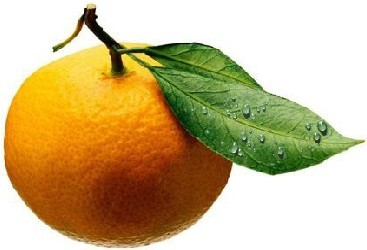
\includegraphics[totalheight=0.22\textheight]{imagenes/mandarina.jpg} %porcentajes de una longitud
%dirección de la imagen respecto al directorio raiz del .tex
\caption{\small  Esta es una figura de ejemplo }
\label{mandarina} 
\end{figure}


Faltaron las integrales y derivadas!
\begin{equation}
    \int_a^b f(x) dx = F(b)-F(a)
\end{equation}



%\begin{figure}[h]
%\centering %centra la imagen
%\includegraphics[width=0.82\textwidth]{cartel1.jpg} %porcentajes de una longitud
%dirección de la imagen respecto al directorio raiz del .tex
%\caption{\small  Esta es otra figura de ejemplo }
%\label{publicidad} 
%\end{figure}

Una vez que creamos una figura, podemos referenciarla . Yo referencio \ref{publicidad} (como vemos en la figura \ref{mandarina}, las mandarinas se parecen a las naranjas). Una ventaja del \LaTeX{} es que si agregamos nuevas figuras o cambiamos el orden, la numeración se arregla sola.

Ahora ya sabemos bastante sobre como escribir y poner figuras. Vamos a hacer algo de matemática

\clearpage  % empezamos una nueva página!

\section{Matem\'atica en \LaTeX{} }

El \LaTeX proporciona un medio superior para escribir matemática. Podemos querer escribir matemática dentro de un párrafo ($e=mc^{2}$) o bien equivalentemente, \begin{math} e = mc^{2} \end{math}. Por otra parte, podemos querer darle un rol un poco más ``central'' a nuestra ecuación, 

\begin{displaymath} 
4345^4 + 345^{4^2} = 5321^{4}
\end{displaymath}

\[4345^{\sqrt[3]{2}}\]

En muchos casos queremos tener nuestras ecuaciones numeradas para referenciarlas luego,

\begin{equation}
\label{ecuacion}
\sum_{n=1}^{\infty} \frac{1}{n^{2}} = \frac{\pi^{2}}{6}
\end{equation}

Entonces, podemos venir y decir (\ldots de acuerdo a la ecuación \ref{ecuacion} \ldots).

Mi gran problema es escribir las ecuación chica en el texto $\Omega = 2 \pi \omega$.

La producción de matemática con \LaTeX{} es un asunto muy vasto. El usuario que quiera profundizar terminará irremediablemente enganchado generando expresiones bellas para la matemática que necesite escribir. 

Por último, para los más matemáticos, podemos crear teoremas, definiciones, demostraciones, y referenciarlos.

\begin{godel}[Incompletitud de Gödel]
Toda teoría formal recursiva que contenga la aritmética elemental no puede ser consistente y completa a la vez. En particular, si es una teoría consistente, existe un enunciado verdadero pero indemostrable dentro de la teoría.
\end{godel}

\begin{godel}
La propiedad de completitud de una teoría no es enunciable dentro de la misma teoría.
\end{godel}

\clearpage

\section{Tablas}

El \LaTeX{} también permite escribir tablas, aunque son un tanto complicadas. Algunos editores proporcionan métodos con una interfaz gráfica más simple. Estos consisten simplemente en rellenar una tabla base y el editor se encarga de traducirlo al código. A continuación presentamos dos ejemplos de distinta dificultad.
\vspace{5mm}

\begin{center} %para centrar
\begin{tabular}{ l | c || r} %para empezar la tabla, l(izquierda), c(centrar), r(derecha) son para decir la cantidad de columnas y si el texto estara centrado o corrido hacia algun lado. Las lineas verticales indican el tipo de separacion entre columnas.
  \hline  %para poner la linea horizontal
  1 & 2 & 3 \\ %& sirve para separar celdas consecutivas y el \\ sirve para saltar a la fila de abajo
  4 & 5 & 6 \\
  7 & 8 & 9 \\
  \hline  
\end{tabular}
\end{center}

\vspace{5mm}

\begin{center}
\begin{tabular}{ |l|l|l| }
\hline
\multicolumn{3}{ |c| }{Team sheet} \\ %multi es para fusionar columnas (multicolumn) o filas (multirow), seguido de la cantidad de filas o columnas entre llaves. A continuacion, para el caso de las columnas se indica la alinieacion y, para el caso de las filas, se indica el ancho. Finalmente, y entre llaves, se indica el contenido.
\hline
Goalkeeper & GK & Paul Robinson \\ \hline
\multirow{4}{*}{Defenders} & LB & Lucus Radebe \\
 & DC & Michael Duberry \\
 & DC & Dominic Matteo \\
 & RB & Didier Domi \\ \hline
\multirow{3}{*}{Midfielders} & MC & David Batty \\
 & MC & Eirik Bakke \\
 & MC & Jody Morris \\ \hline
Forward & FW & Jamie McMaster \\ \hline
\multirow{2}{*}{Strikers} & ST & Alan Smith \\
 & ST & Mark Viduka \\
\hline
\end{tabular}
\end{center}
%que pasara si vamos sacando distintas lineas?

Estas tablas se pueden referenciar de la misma forma que las imágenes.

\section{Y las referenecias?}

Para hacer informes uno suele contar con la ayuda de la agrupación que más te gusta\cite{fifa}, la mejor página web de la historia \cite{google} y a veces algún libro\cite{yosoyeldiego}. Y ojo, que a veces también vas a querer citar un paper\cite{paper}.

\begin{thebibliography}{99}
% el {99} indica el número máximo de referencias que podés poner, claro que si lo cambiás podés poner más (o menos)

\bibitem{fifa}
  La FIFA,
  \emph{\LaTeX{}: Para todos los pibitos y las pibitas piola},
  Ed. Sin Presupuesto, Buenos Aires,
  No Llevamos la cuenta de las ediciones,
  2016.

\bibitem{google}
    \href{https://www.google.com}{Google}

\bibitem{yosoyeldiego}
    \emph{Yo Soy El Diego},
    Ed. Planeta,
    2002.

\bibitem{paper}
    J. C. Maxwell. \textbf{Phil. Trans. R. Soc. Lond.} 1 January 1865 \textbf{vol. 155} 459-512
\end{thebibliography}

\end{document}    % cada vez que abrimos un environment, debemos cerrarlo.



